\begin{enumerate}
	\item Exercício
		
	\begin{equation*}
		x^2 + y^2 = r^2 = 2^2 = 4
	\end{equation*}
	\begin{equation*}
		0 \leq r \leq 2,\, 0 \leq \theta \leq 2\pi,\, 0 \leq z \leq 5	
	\end{equation*}
	
	\begin{figure}[htb]
		\caption{Coordenadas cilíndricas - Aula 02 - Exercício I}
		\label{v26_a02_e01}
		\centering
		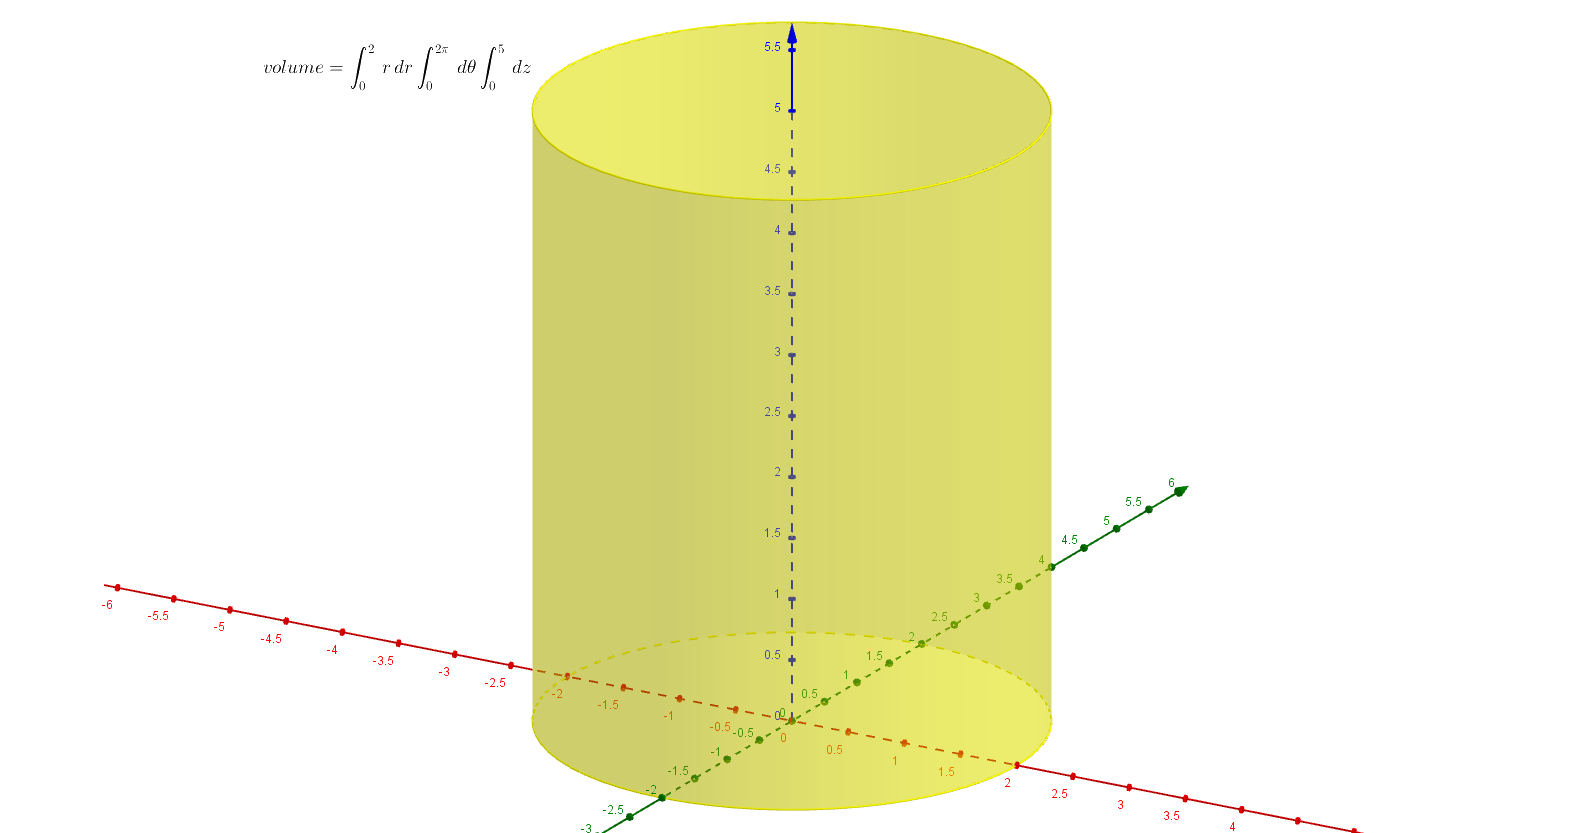
\includegraphics[width=0.5\textwidth]{v26_a02_e01.png}		
	\end{figure}
	
	\begin{gather*}
		\int_0^2 r\, dr \int_0^{2\pi} d\theta \int_0^5 dz = \left[\dfrac{r^2}{2}\right]_0^2 \left[\theta\right]_0^{2\pi} \left[z\right]_0^5 = \dfrac{4}{\overstrike{2}}\overstrike{2}\pi 5 = 20\pi 
	\end{gather*}
	
\end{enumerate}